% Preface — From Token to Fleet: An AI Solution Architect's Handbook

For a long time I wanted to build the systematic knowledge of what it means
to work as an AI Solution Architect: how to reason across the layers of an
AI system --- from tokens and models to workloads, systems, infrastructure,
and fleets --- so that a vague requirement can be turned into a defensible
architecture. I kept looking for the resource that would lay all of that
down in one coherent thread. What I found were deep dives into single
layers --- models, serving, infrastructure, agents --- but no single spine
that connected them into the one thing an architect actually does: chaining
a real workload to a defensible solution.

Eventually I realized that the best way for me to build that knowledge was to
go through the development journey myself, and that writing it down is how
the knowledge gets built. I am not writing from a finished body of expertise;
I am documenting a body of knowledge as I learn it, chapter by chapter, and
I will keep updating these pages as I learn about new AI technologies. The
moment I try to write down how I would decide whether a model belongs on a
particular accelerator, I am forced to make explicit --- parameter count,
active parameters, KV-cache, context length, quantization, memory bandwidth,
compute intensity, batching, interconnect, latency, throughput, concurrency,
cost, reliability --- every quantity that connects the model to the workload.
And the act of writing exposes the holes in my own understanding, which
tells me what I still need to learn next.

That feedback loop --- curiosity, question, research, model, write, discover
a gap, new question --- is the engine of this book.

The AI field moves fast, and I am still learning too. This book is my
learning notes, shared --- written the only way I know: layer by layer,
decision by decision, from the token up to the fleet. If it helps others who
are interested in the AI Solution Architect role build the same systematic
mental model, then it has outdone what I had planned it for. Learning is a
proactive act; curiosity is the ultimate driver.

\section*{The thesis}

The book has one thesis, and it is the spine of every chapter:

\begin{quote}
\textbf{Given an ambiguous problem, how do I systematically arrive at a
defensible AI architecture?}
\end{quote}

The canonical method --- the decision loop that Chapter~22 makes explicit
and every chapter echoes --- runs from requirements and workload
characterization, through constraints and candidate architectures, to
benchmarking, bottleneck analysis, optimization, total-cost reality checks,
and a final red-team challenge. Parts~I--V walk through the technical
substrate, layer by layer. Part~VI turns to the discipline itself: how one
learns to reason across those layers.

\begin{figure}[htbp]
  \centering
  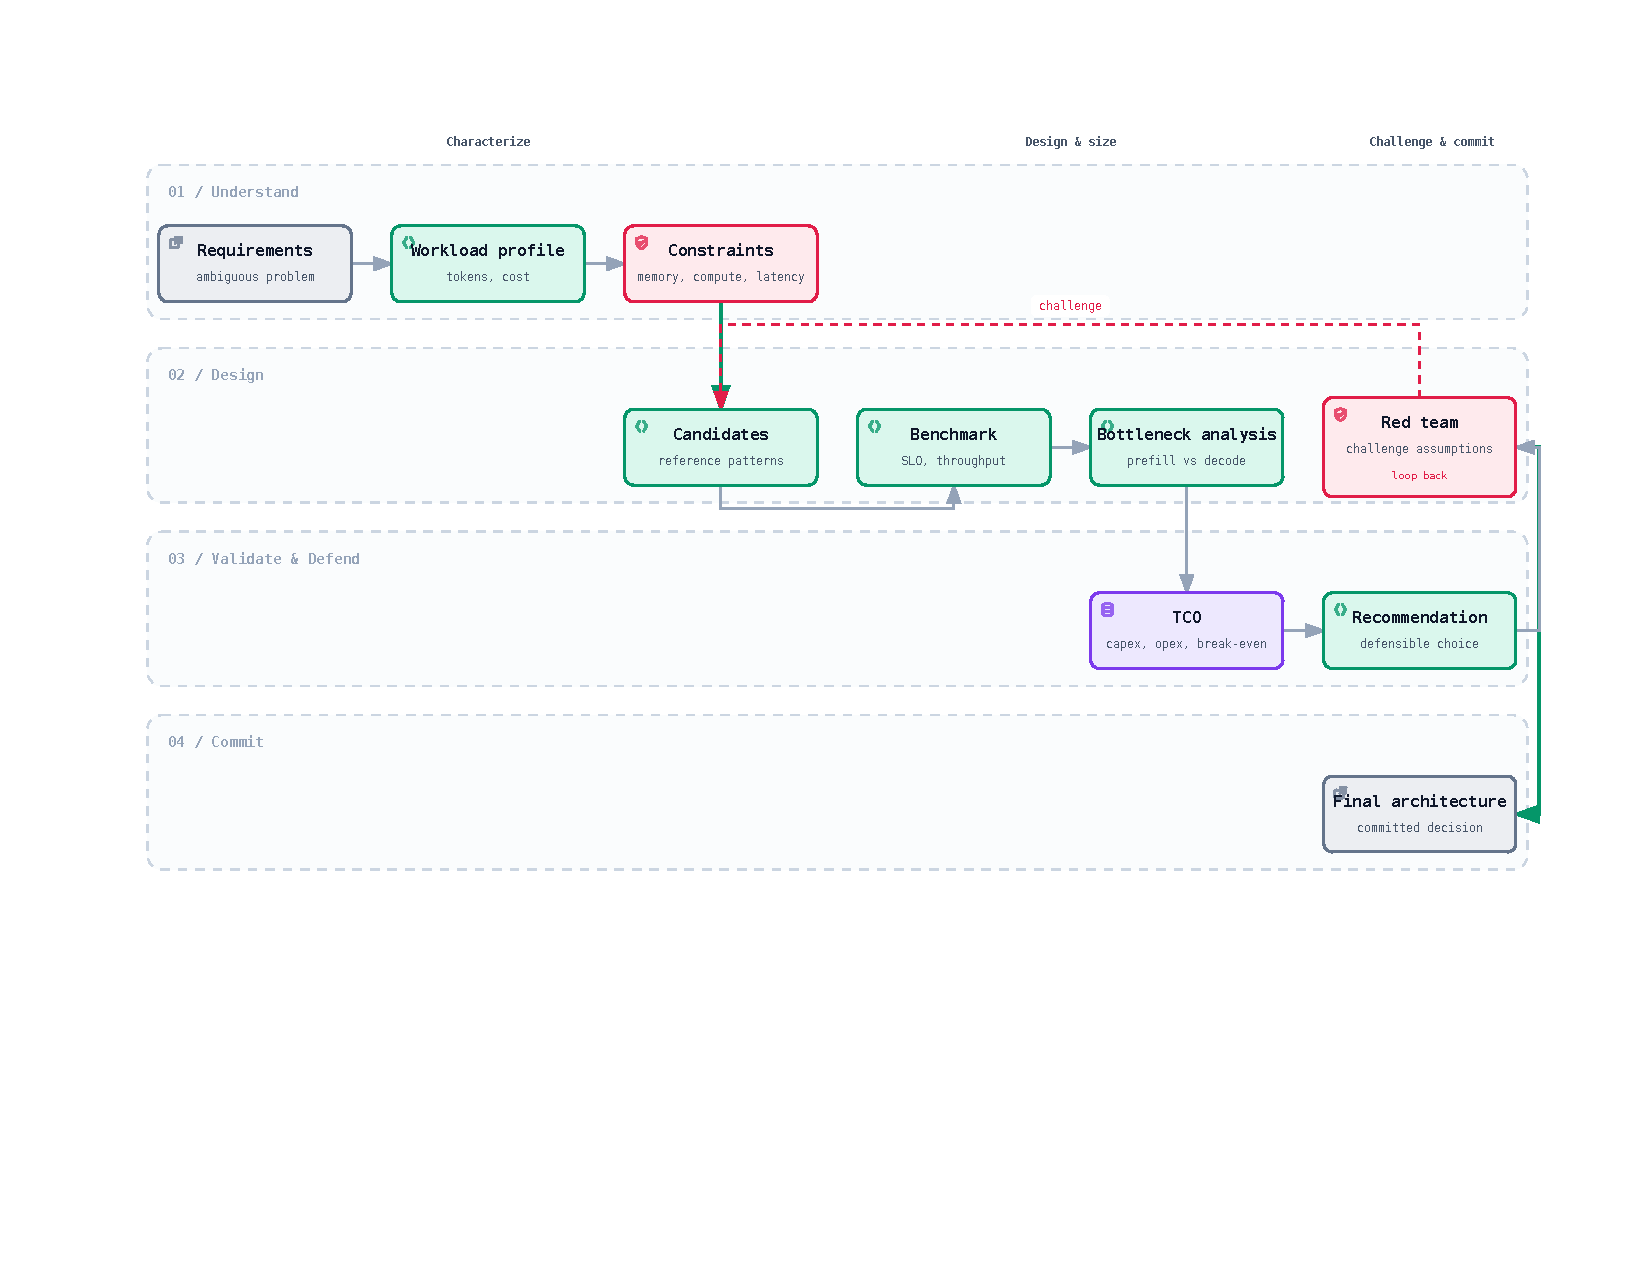
\includegraphics[width=\maxwidth{\textwidth},keepaspectratio]{assets/spine-decision-loop.pdf}
  \caption{The architect's decision loop --- the book's spine. A vague
  requirement is carried through workload characterization, constraints,
  candidate architectures, benchmarking, bottleneck analysis, TCO, and a
  final red-team challenge before an architecture is committed. [ILLUSTRATIVE conceptual]}
  \label{fig:spine-loop}
\end{figure}

\section*{How the book is organized}

The six parts mirror the layers an architect reasons across:

\begin{itemize}
  \item \textbf{Part I --- The Token.} Models and mechanisms, from a single
token to the memory and compute arithmetic that prices every decision.
  \item \textbf{Part II --- The Workload.} The job the system does: workload
characterization and measuring what matters.
  \item \textbf{Part III --- The System.} Memory, compute, communication,
parallelism, and serving.
  \item \textbf{Part IV --- The Architecture.} Designing, benchmarking,
engineering, and costing a system.
  \item \textbf{Part V --- The Fleet.} Operating AI at scale, and agents.
  \item \textbf{Part VI --- The Architect.} The spine made explicit, plus a
patterns library.
\end{itemize}

\begin{figure}[htbp]
  \centering
  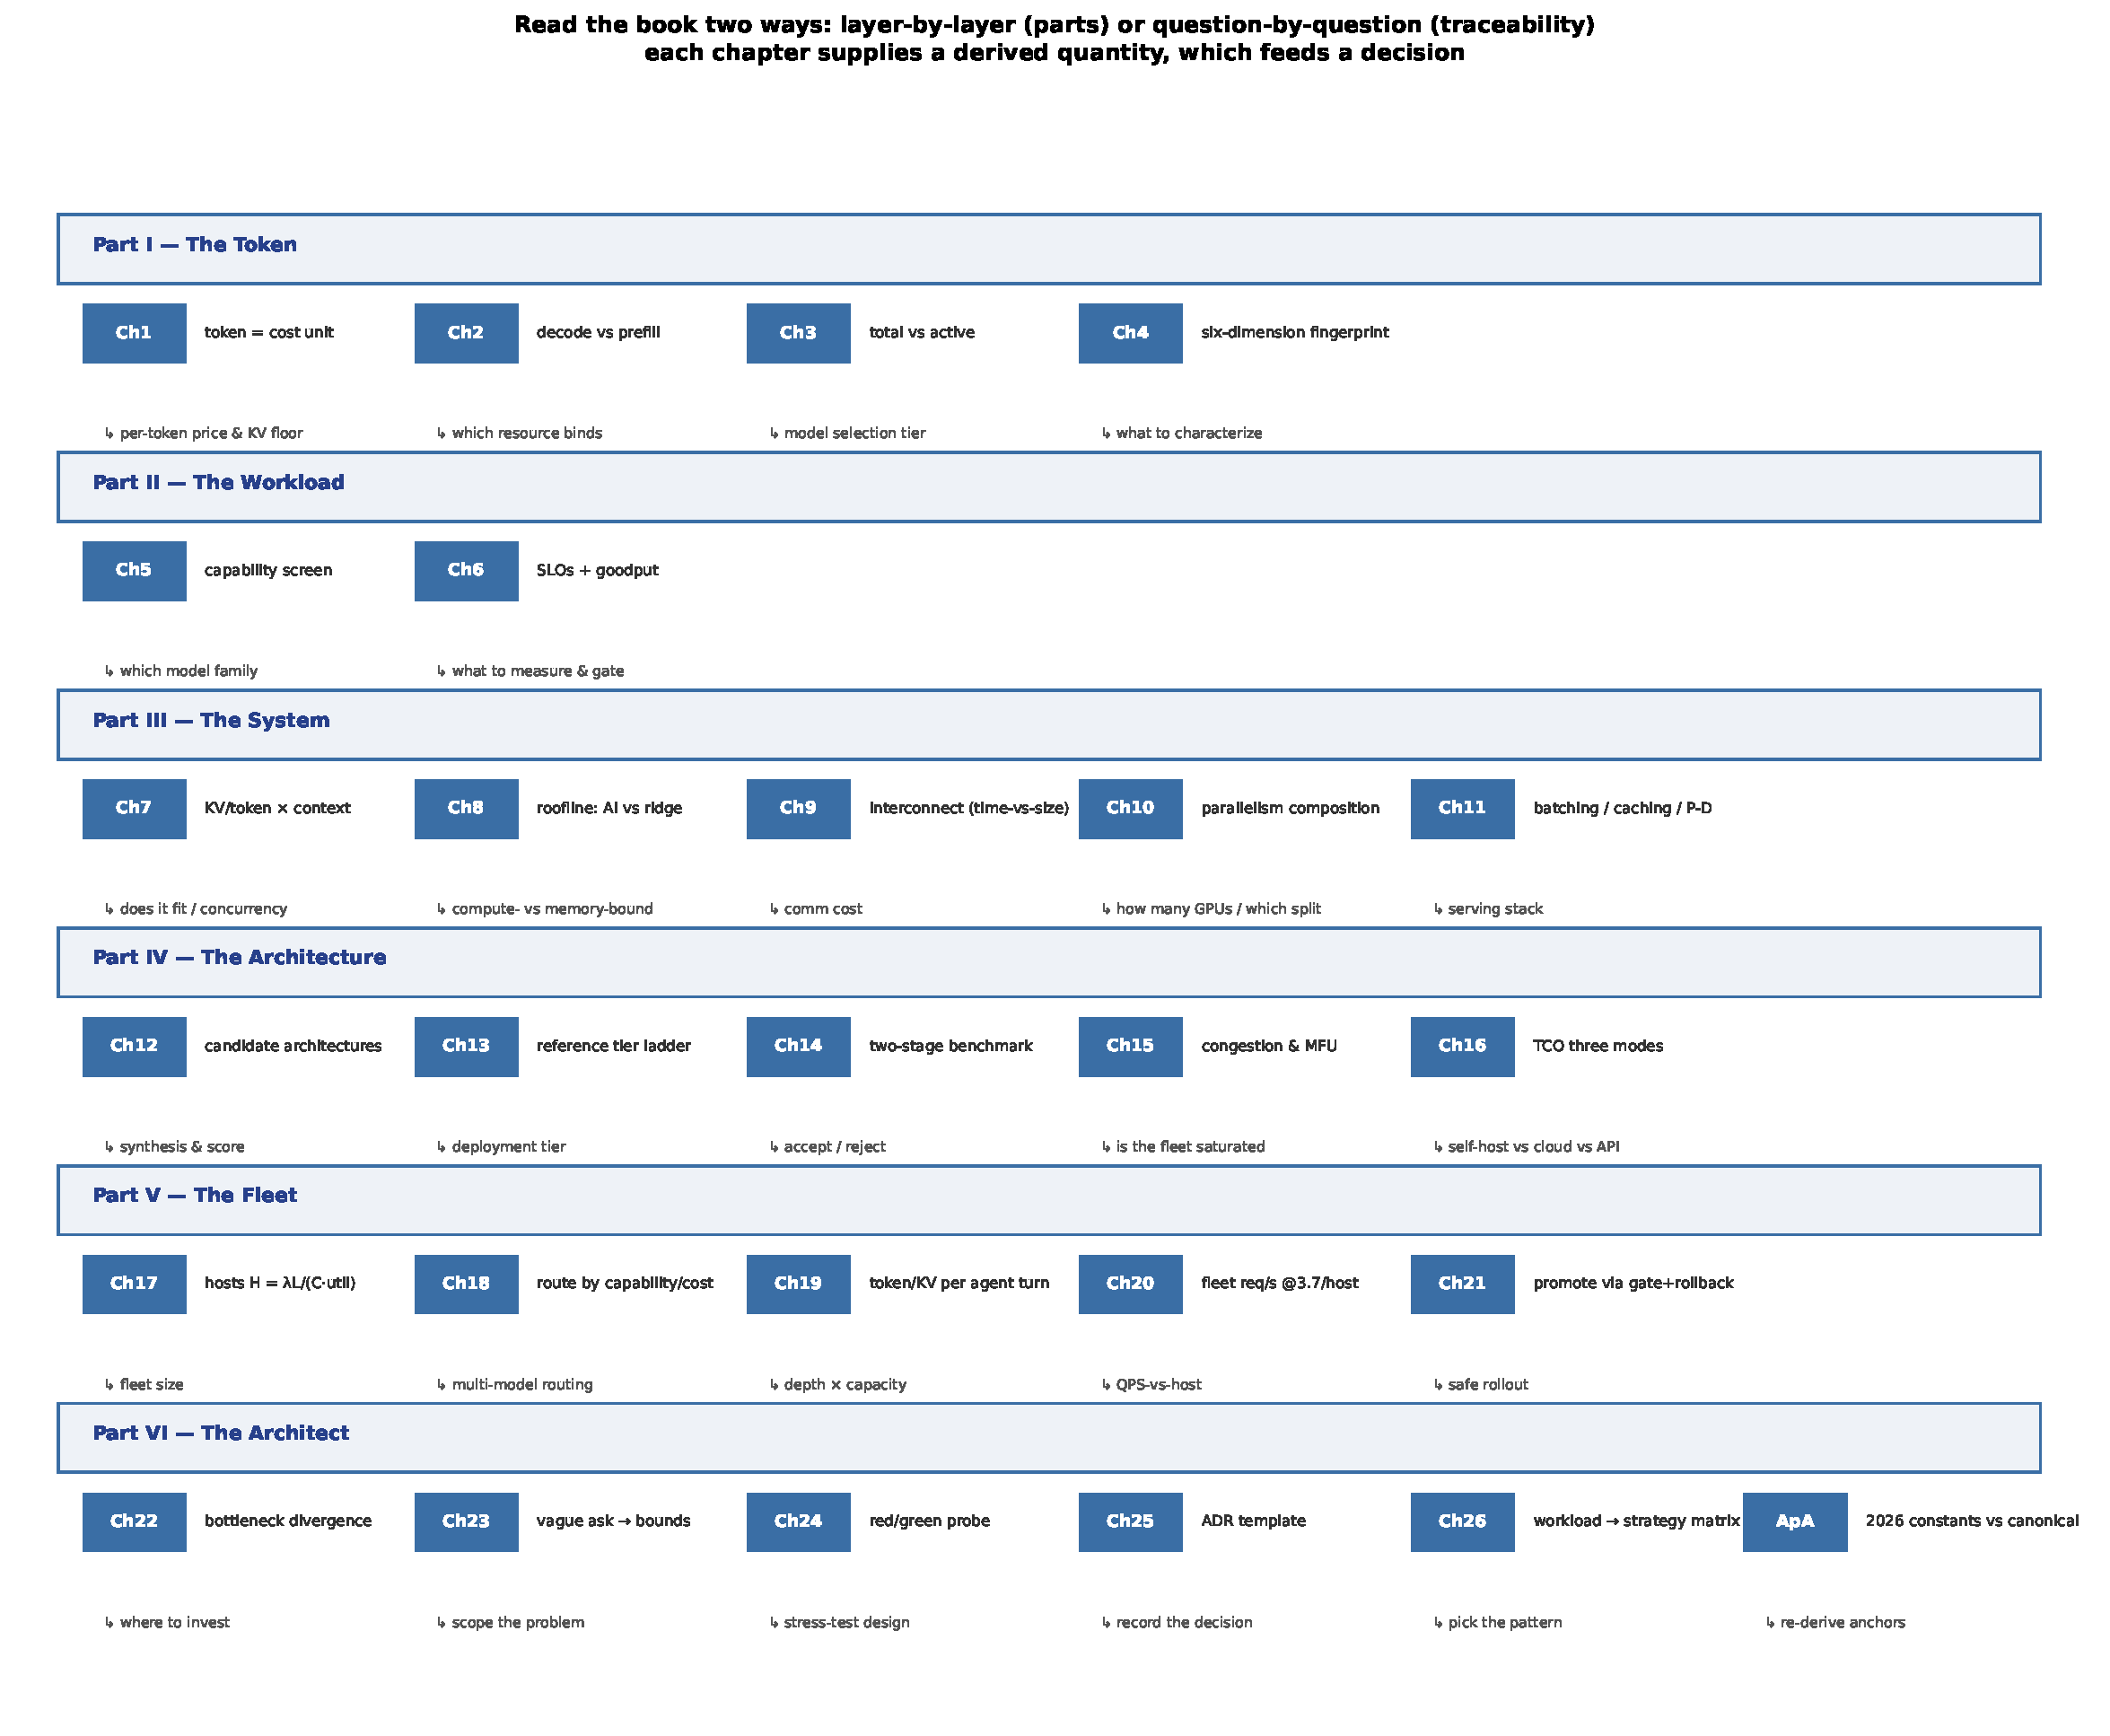
\includegraphics[width=\maxwidth{\textwidth},keepaspectratio]{assets/preface-trace.pdf}
  \caption{Reading the book by number. Each chapter supplies a derived quantity --- a token/KV floor, a roofline point, a fleet size --- and that quantity feeds a decision. Reading down a Part's strip gives the layer-by-layer thread; reading across any chapter's chip shows which number to reach for to answer a given question. [ILLUSTRATIVE]}
  \label{fig:traceability}
\end{figure}

A worked canonical scenario --- an enterprise retrieval-augmented question-answering
workload on a 70B-class model --- runs through the book, so every mechanism is
anchored in concrete, reproducible arithmetic rather than abstraction. One caveat, so
the book is not misread: this scenario is a \textbf{teaching instrument}, not a claim
about what an AI workload \emph{is}. Real workloads span a wide design space ---
long-context RAG (KV/memory-bound), high-throughput chat (decode-bound), batch
inference (utilization/cost-bound), reasoning (test-time-compute-bound), agentic
(concurrency/variance-bound), embeddings, vision, fine-tuning, training --- and each
shifts which quantity dominates. The canonical scenario picks a single, tractable,
input-heavy RAG case and carries it through so the reasoning stays continuous; a real
deployment will sit somewhere else in that space, and the chapters are written to
give the reader the arithmetic to re-derive the bounds for \emph{their} point.

\section*{The Architect's Evidence Discipline}

Every quantitative claim in this book carries two orthogonal labels, and
keeping these axes separate is itself a discipline. The \textbf{source} axis
records where the number came from: \textbf{[1P]} first-party (the model
vendor's own spec), \textbf{[2°]} reputable second-hand (textbook, survey,
independent benchmark), or \textbf{[VERIFY]} not yet anchored. The
\textbf{claim-type} axis records what was done to it: \textbf{FACT} directly
stated by the source, \textbf{DERIVED} computed from documented facts,
\textbf{HYPOTHESIS} reasoned but not yet validated, or \textbf{ILLUSTRATIVE}
--- a round, teaching number chosen to make a mechanism concrete, never a
measured or stable fact. Home-lab experiments are not reference. Where a
figure is a vendor-reported claim, it is flagged, and the verification step
is described so a reader can check it on their own hardware.

Two habits matter most. First, arithmetic belongs on the claim-type axis, not
the source axis: a worked example computed from a model card is \textbf{[1P]
DERIVED}, never \textbf{[2°]} just because arithmetic was done. Second, the
conclusions an architect draws are only as defensible as the units behind
them --- so every major worked example ends with a unit check and a sanity
check (does this result stay inside the physically possible?). That habit is
part of the discipline, not an appendix.

\section*{Reading conventions}

Three conventions keep the book consistent and honest about its own limits.

\textbf{Terminology.} A few nouns are used as synonyms for readability: HBM,
VRAM and GPU memory name the same physical resource; TTFT,
time-to-first-token and prefill latency likewise; RAG and
retrieval-augmented-\-generation are the same. Where a distinction is
architecturally load-bearing --- prefill versus decode, total versus active
parameters, model capacity versus system capacity --- the book holds it
sharply. Synonyms are a readability concession; load-bearing contrasts are
never relaxed (Ch.~2, 8, 17).

\textbf{Hardware is a generic stand-in.} The worked arithmetic is anchored to
concrete constants (e.g. an 8\texttimes H100 host at roughly 1 PFLOPS FP16
and ~3.4 TB/s HBM) because arithmetic needs concrete anchors. Those values
are a \emph{current} high-end accelerator, presented as an example, not a
prophecy: the H200, B100/B200 and later generations change the constants, not
the method. Re-derive the constants from the current hardware sheet; the
roofline (Ch.~8) and the canonical arithmetic (Ch.~7) keep the method
independent of any single generation. Forward-looking numbers are marked
ILLUSTRATIVE.

\textbf{Quick reference.} For a day-to-day cheat-sheet: Chapter~26 (\S2.1)
carries a workload-to-strategy decision matrix, and Chapter~25's Architecture
Decision Record is a reusable template to copy into a repository. Those, plus
the evidence discipline above, are worth re-reading first whenever a chapter
feels dense.

\section*{A note on currency}

The mechanisms in this handbook --- tokens, memory floors, rooflines,
parallelism, KV arithmetic --- are durable; they do not change as the
industry moves. But the frontier does move, and a handbook for architects
should carry the latest technology information. The Appendix therefore
surveys the frontier open-weight architectures of 2026, mapped back to the
mechanisms and decisions explored in the body of the book --- and closes on
the question that is more durable than any single architecture: \emph{where
should the intelligence live}.
